\chapter{Vectors}

We have talked a some about forces, but in the calculations that we
have done, we have only talked about the magnitude of a force. It is
equally important to talk about its direction. To do the math on
things with a magnitude and a direction (like forces), we need vectors.\index{vectors}

For example, if you jump out of a plane (hopefully with a parachute), 
several forces with different magnitudes and directions will be acting upon 
you. Gravity will push you straight down. That force will be proportional to your weight.
If there were a wind from the west, it would push you toward the east. That force
will be proportional to the square of the speed of the wind and approximately proportional to 
your size. Once you are falling, there will be resistance from the air 
that you are pushing through --- that force will point in the opposite direction
from the direction you are moving and will be proportional to the square of your
speed.
% Image added

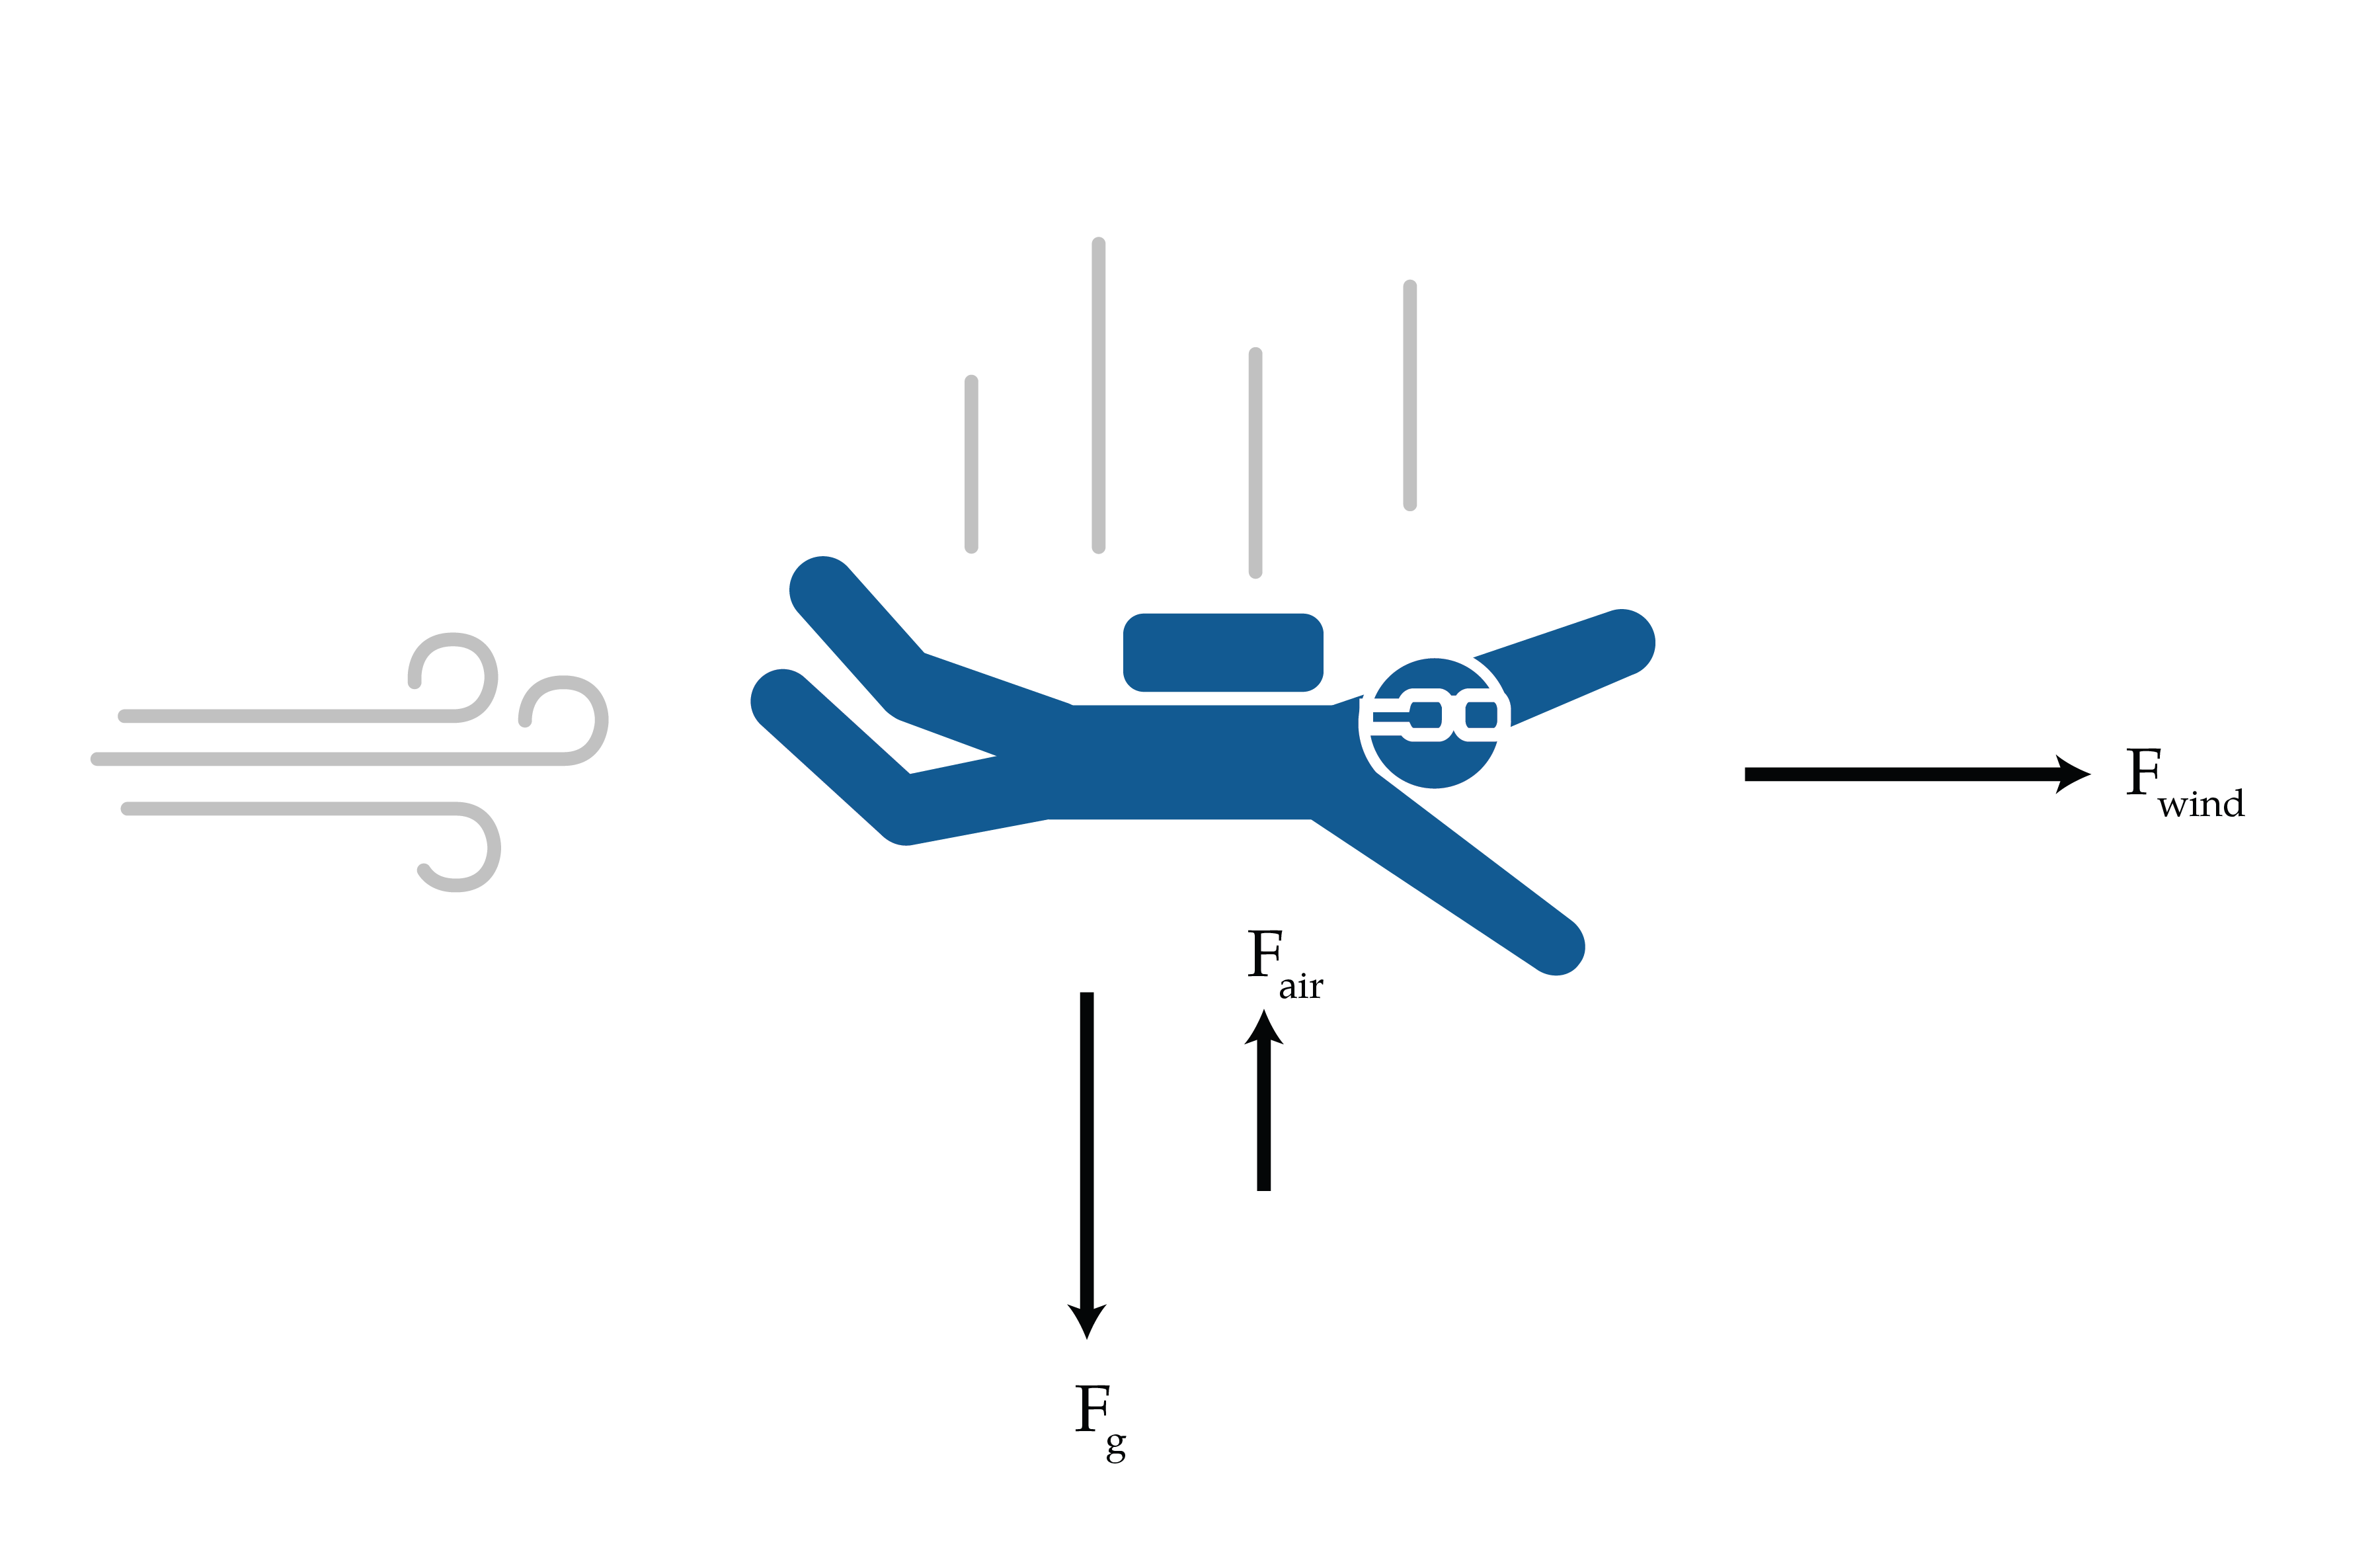
\includegraphics[width=1\textwidth]{skydiver.png}


To figure out the net force (which will tell us how we will accelerate), we will 
need to add these forces together. To do this, we need to learn to do math with vectors.

\section{Adding Vectors}

A vector is typically represented as a list of numbers, with each
number representing a particular dimension. For example, if you are
creating a 3-dimensional vector representing a force, it will have
three numbers representing the amount of force in each of the three
axes. For example, if a force of one newton is in the direction of the
$x$-axis, you might represent the vector as $v = [1, 0, 0]$. 
Another vector might be $u = [0.5, 0.9, 0.7]$ \index{vectors!adding}.

\tdplotsetmaincoords{80}{130} 
\begin{tikzpicture} [scale=4, tdplot_main_coords, axis/.style={->,sdkblue}, 
vector/.style={-stealth,black,very thick}, 
vector guide/.style={dashed,sdkblue}]

%standard tikz coordinate definition using x, y, z coords
\coordinate (O) at (0,0,0);

%draw axes
\draw[axis] (0,0,0) -- (1.5,0,0) node[anchor=north east]{$x$};
\draw[axis] (0,0,0) -- (0,0.9,0) node[anchor=north west]{$y$};
\draw[axis] (0,0,0) -- (0,0,0.9) node[anchor=south]{$z$};

%draw a vector from O to P
\draw[vector] (O) -- (1,0,0);
\draw[vector] (O) -- (0.5,0.9,0.7);
\draw (0.2,0.0,0.05) node[left] {v};
\draw (0.2,0.35,0.3) node[right] {u};

\draw[vector guide] (0.5,0,0) -- (0.5,0.9,0);
\draw[vector guide] (0.0,0.9,0) -- (0.5,0.9,0);
\draw[vector guide] (0.5,0.9,0) -- (0.5,0.9,0.7);
\end{tikzpicture}

Thinking visually, when we add to vectors, we put the starting point 
second vector at the ending point of the first vector.


\tdplotsetmaincoords{80}{130} 
\begin{tikzpicture} [scale=4, tdplot_main_coords, axis/.style={->,sdkblue}, 
light vector/.style={-stealth,dashed,very thick, black}, 
vector/.style={-stealth,black,very thick}, 
vector guide/.style={dashed,sdkblue}]

%standard tikz coordinate definition using x, y, z coords
\coordinate (O) at (0,0,0);

%draw axes
\draw[axis] (0,0,0) -- (1.5,0,0) node[anchor=north east]{$x$};
\draw[axis] (0,0,0) -- (0,0.9,0) node[anchor=north west]{$y$};
\draw[axis] (0,0,0) -- (0,0,0.9) node[anchor=south]{$z$};

%draw a vector from O to P
\draw[light vector] (0,0,0) -- (0.5,0.9,0.7);
\draw[light vector] (0.5, 0.9, 0.7) -- (1.5, 0.9, 0.7);
\draw[vector] (0,0,0) -- (1.5,0.9,0.7) node[left] {u + v};
\draw (0.7,0.9,0.75) node[left] {v};
\draw (0.2,0.35,0.3) node[right] {u};

\draw[vector guide] (0.5,0,0) -- (0.5,0.9,0);
\draw[vector guide] (0.0,0.9,0) -- (0.5,0.9,0);
\draw[vector guide] (0.5,0.9,0) -- (0.5,0.9,0.7);
\draw[vector guide] (0.5,0.9,0) -- (1.5,0.9,0.0);
\draw[vector guide] (1.5,0.9,0.0) -- (1.5,0.9,0.7);
\draw[vector guide] (1.5,0.0,0.0) -- (1.5,0.9,0.0);

\end{tikzpicture}

If you know the vectors, you will just add them element-wise:

$$ u + v = [0.5, 0.9, 0.7] + [1.0, 0.0, 0.0] = [1.5, 0.9. 0.7] $$

These vectors have 3 components, so we say they are \newterm{3-dimensional}. 
Vectors can have any number of components. For example, the vector
 $[-12.2, 3, \pi, 10000]$ is 4-dimensional.

 You can only add two vectors if they have the same dimension.

 $$ [12, -4] + [-1, 5] = [11,1] $$

 Addition is commutative; if you have two vectors $a$ and $b$, then
 $a + b$ is the same as $b + a$.

 Addition is also associative: If you have three vectors $a$, $b$, and $c$,
 it doesn't matter which order you add them in. 
 That is, $a + (b + c) = (a + b) + c$.

 A 1-dimensional vector is just a number. We say it is a 
 \newterm{scalar}, not a vector.

 \begin{Exercise}[title={Adding vectors}, label=adding_vectors]
Add the following vectors:
\begin{itemize}
    \item $[1, 2, 3] + [4, 5, 6]$
    \item $[-1, -2, -3, -4] + [4, 5, 6, 7]$
    \item $[\pi, 0, 0] + [0, \pi, 0] + [0, 0, \pi]$
\end{itemize}
\end{Exercise}
\begin{Answer}[ref=adding_vectors]
    \begin{itemize}
        \item $[1, 2, 3] + [4, 5, 6] = [5, 7, 9]$
        \item $[-1, -2, -3, -4] + [4, 5, 6, 7] = [3, 3, 3, 3]$
        \item $[\pi, 0, 0] + [0, \pi, 0] + [0, 0, \pi] = [\pi, \pi, \pi]$ 
    \end{itemize}
\end{Answer}

    \begin{Exercise}[title={Adding Forces}, label=adding_forces]
        You are adrift in space, near two different stars. 
        The gravity of one star is pulling you towards it with a 
        force of $[4.2, 5.6, 9.0]$ newtons.
        The gravity of the other star is pulling you towards it with
        a force of $[-100.2, 30.2, -9.0]$ newtons. What is the net force?
        \end{Exercise}
        \begin{Answer}[ref=adding_forces]
            To get the net force, you add the two forces:

            $$F = [4.2, 5.6, 9.0] + [-100.2, 30.2, -9.0] = [-96, 35.8, 0.0] \text{ newtons}$$
   
\end{Answer}

\section{Multiplying a vector with a scalar}

It is not uncommon to multiply a vector by a scalar. For example, a rocket engine
might have a force vector $v$. If you fire 9 engines in the exact same direction,
the resulting force vector would be $9v$.\index{vectors!multipying by a scalar}

Visually, when we multiply a vector $u$ by a scalar $a$, we get a new vector that
goes in the same direction as $u$ but has a magnitude $a$ times as long as $u$.

\tdplotsetmaincoords{80}{130} 
\begin{tikzpicture} [scale=3, tdplot_main_coords, axis/.style={->,sdkblue}, 
vector/.style={-stealth,black,very thick}, 
vector guide/.style={dashed,sdkblue}]

%standard tikz coordinate definition using x, y, z coords
\coordinate (O) at (0,0,0);

%draw axes
\draw[axis] (0,0,0) -- (1.6,0,0) node[anchor=north east]{$x$};
\draw[axis] (0,0,0) -- (0,2.8,0) node[anchor=north west]{$y$};
\draw[axis] (0,0,0) -- (0,0,1.9) node[anchor=south]{$z$};

%draw a vector from O to P
\draw[vector] (O) -- (0.5,0.9,0.7);
\draw (0.2,0.35,0.3) node[right] {$u$};

\draw[vector] (O) -- (1.5,2.7,2.1) node[right] {$3u$};


\draw[vector guide] (0.5,0,0) -- (0.5,0.9,0);
\draw[vector guide] (0.0,0.9,0) -- (0.5,0.9,0);
\draw[vector guide] (0.5,0.9,0) -- (0.5,0.9,0.7);

\draw[vector guide] (1.5,0,0) -- (1.5,2.7,0);
\draw[vector guide] (0.0,2.7,0) -- (1.5,2.7,0);
\draw[vector guide] (1.5,2.7,0) -- (1.5,2.7,2.1);
\end{tikzpicture}

When you multiply a vector by a scalar, you simply multiply each of the components by the scalar:

$$ 3 \times [0.5, 0.9, 0.7] = [1.5, 2.7, 3.6] $$

\begin{Exercise}[title={Multiplying a vector and a scalar}, label=mult_scalar]
    Simplify the following expressions:
    \begin{itemize}
        \item $2 \times [1, 2, 3]$
        \item $[-1, -2, -3, -4] \times -2$
        \item $\pi[\pi, 2\pi, 3\pi]$
    \end{itemize}
    \end{Exercise}
    \begin{Answer}[ref=mult_scalar]
        \begin{itemize}
            \item $2 \times [1, 2, 3] = [2, 4, 6]$
            \item $[-1, -2, -3, -4] \times -3 = [3, 6, 9, 12]$
            \item $\pi[\pi, 2\pi, 3\pi]  = \pi^2, 2\pi^2, 3\pi^2]$ 
        \end{itemize}
    \end{Answer}

Note that when you multiply a vector times a negative number, the new vector points 
in the opposite direction.

\tdplotsetmaincoords{80}{130} 
\begin{tikzpicture} [scale=5, tdplot_main_coords, axis/.style={->,sdkblue}, 
vector/.style={-stealth,black,very thick}, 
vector guide/.style={dashed,sdkblue}]

%standard tikz coordinate definition using x, y, z coords
\coordinate (O) at (0,0,0);

%draw axes
\draw[axis] (0,0,0) -- (0.55,0,0) node[anchor=north east]{$x$};
\draw[axis] (0,0,0) -- (0,0.95,0) node[anchor=north west]{$y$};
\draw[axis] (0,0,0) -- (0,0,0.6) node[anchor=south]{$z$};

%draw a vector from O to P
\draw[vector] (O) -- (0.5,0.9,0.7);
\draw (0.2,0.36,0.3) node[right] {$u$};

\draw[vector] (O) -- (-0.25,-0.45,-0.35) node[right] {$(-0.5)u$};

\draw[vector guide] (0.5,0,0) -- (0.5,0.9,0);
\draw[vector guide] (0.0,0.9,0) -- (0.5,0.9,0);
\draw[vector guide] (0.5,0.9,0) -- (0.5,0.9,0.7);

\draw[vector guide] (-0.25,0,0) -- (-0.25,-0.45,0);
\draw[vector guide] (0,0,0) -- (-0.25,0,0);
\draw[vector guide] (0.0,-0.45,0) -- (-0.25,-0.45,0);
\draw[vector guide] (0,0,0) -- (0,-0.45,0);

\draw[vector guide] (-.25,-0.45,0) -- (-0.25,-0.45,-0.35);
\end{tikzpicture}

\section{Vector Subtraction}

As you might guess, when you subtract one vector from another, 
you just do element-wise subtraction:\index{vectors!subtraction}

$$[4,2,0] - [3,-2, 9] = [1, 4, -9]$$

So, $u - v = u + (-1v)$.

Visually, you reverse the one that is being subtracted:


\tdplotsetmaincoords{80}{130} 
\begin{tikzpicture} [scale=5, tdplot_main_coords, axis/.style={->,sdkblue}, 
light vector/.style={-stealth,dashed,very thick, black}, 
vector/.style={-stealth,black,very thick}, 
vector guide/.style={dashed,sdkblue}]

%standard tikz coordinate definition using x, y, z coords
\coordinate (O) at (0,0,0);

%draw axes
\draw[axis] (0,0,0) -- (0.55,0,0) node[anchor=north east]{$x$};
\draw[axis] (0,0,0) -- (0,1.0,0) node[anchor=north west]{$y$};
\draw[axis] (0,0,0) -- (0,0,0.75) node[anchor=south]{$z$};

%draw a vector from O to P
\draw[light vector] (0,0,0) -- (0.5,0.9,0.7);
\draw[light vector] (0.5, 0.9, 0.7) -- (-0.5, 0.9, 0.7);
\draw[vector] (0,0,0) -- (-0.5,0.9,0.7) node[right] {u - v};
\draw (0.1,0.9,0.75) node[left] {-v};
\draw (0.29,0.34,0.32) node[right] {u};

\draw[vector guide] (0.5,0,0) -- (0.5,0.9,0);
\draw[vector guide] (0.0,0.9,0) -- (0.5,0.9,0);
\draw[vector guide] (0.5,0.9,0) -- (0.5,0.9,0.7);
\draw[vector guide] (0.5,0.9,0) -- (-0.5,0.9,0.0);
\draw[vector guide] (-0.5,0.9,0.0) -- (-0.5,0.9,0.7);
\draw[vector guide] (-0.5,0.0,0.0) -- (-0.5,0.9,0.0);
\draw[vector guide] (0,0.0,0.0) -- (-0.5,0.0,0.0);

\end{tikzpicture}

\section{Magnitude of a Vector}

The \newterm{magnitude} of a vector is just its length. We write the 
magnitude of a vector $v$ as $|v|$.\index{vectors!magnitude of}

We compute the magnitude using the pythagorean theorem.  If $v = [3,4,5]$, 
then

\begin{equation*}
    |v| = \sqrt{3^2 + 4^2 + 5^2} = \sqrt{50} \approx 7.07
\end{equation*}

(You might notice that the notation for the magnitude is exactly like the notation for absolute value.
If you think of a scalar as a 1-dimensional vector, the absolute value and the magnitude are the same. 
For example, the absolute value of -5 is 5.  If you take the magnitude of the one-dimenional vector $[-5]$,
you get $\sqrt{25} = 5$.)

Notice that if you scale up a vector, its magnitude scales by the same amount. For example:

\begin{equation*}
|7[3,4,5]| = 7 \sqrt{50} \approx 7 \times 7.07    
\end{equation*}

The rule then is: If you have any vector $v$ and any scalar $a$:
\begin{equation*}
    |a v| = |a| |v|
\end{equation*}


\begin{Exercise}[title={Magnitude of a Vector}, label=vector_mag]
    Find the magnitude of the following vectors:
    \begin{itemize}
        \item $[1, 1, 1]$
        \item $[-5, -5, -5]$ (that is the same as $-5 \times [1, 1, 1]$)
        \item $[3, 4, -4] + [-2, -3, 5]$
    \end{itemize}
    \end{Exercise}
    \begin{Answer}[ref=vector_mag]
        \begin{itemize}
            \item $|[1, 1, 1]| = \sqrt{3} \approx 1.73 $
            \item $|[-5, -5, -5]| = |-5 \times [1,1,1]| = 5 \sqrt{3} \approx 8.66$
            \item $|[3, 4, 5] + [-2, -3, -4]| = | [1,1,1] | = \sqrt{3} \approx 1.73$ 
        \end{itemize}
    \end{Answer}

\section{Vectors in Python}

NumPy is a library that allows you to work with vectors in Python.  
You might need to install it on your computer. This is done with \pyfunction{pip}. 
\pyfunction{pip3} installs things specifically for Python 3.\index{vectors!in python}

\begin{Verbatim}
pip3 install NumPy
\end{Verbatim}

We can think of a vector as a list of numbers.  
There are also grids of numbers known as \newterm{matrices}. NumPy deals with both in the same way, 
so it refers to both of them as arrays.\index{NumPy}

The study of vectors and matrices is known as \newterm{Linear Algebra}. Some of the functions we need
are in a sublibrary of NumPy called \pyfunction{linalg}. \index{linalg}

As a convention, everyone who uses NumPy, imports it as \textit{np}. \index{np}

Create a file called \filename{first\_vectors.py}:

\begin{Verbatim}
import NumPy as np

# Create two vectors
v = np.array([2,3,4])
u = np.array([-1,-2,3])
print(f"u = {u}, v = {v}")

# Add them
w = v + u
print(f"u + v = {w}")

# Multiply by a scalar
w = v * 3
print(f"v * 3 = {w}")

# Get the magnitude
# Get the magnitude
mv = np.linalg.norm(v)
mu = np.linalg.norm(u)
print(f"|v| = {mv}, |u| = {mu}")
\end{Verbatim}

When you run it, you should see:

\begin{Verbatim}
> python3 first_vectors.py
u = [-1 -2  3], v = [2 3 4]
u + v = [1 1 7]
v * 3 = [ 6  9 12]
|v| = 5.385164807134504, |u| = 3.7416573867739413
\end{Verbatim}

\subsection{Formatting Floats}

The numbers 5.385164807134504 and 3.7416573867739413 are pretty long.  You probably want them 
rounded off after a couple of decimal places.

Numbers with decimal places are called \newterm{floats}. In the placeholder for your float, you 
can specify how you want it formatted, including the number of decimal places.

Change the last line to look like this:\index{floats!formatting}
\begin{Verbatim}
    print(f"|v| = {mv:.2f}, |u| = {mu:.2f}")
\end{Verbatim}

When you run the code, it will be neatly rounded off to two decimal places:
\begin{Verbatim}
|v| = 5.39, |u| = 3.74
\end{Verbatim}
